\section{Teorema de Green}

El teorema de Green relaciona una integral de línea alrededor de una curva cerrada con una integral doble sobre la región encerrada. Si un campo plano es $\mathbf{F}=\langle P,Q\rangle$, la integral
\[
\oint_C \mathbf{F}\cdot d\vec r
\]
mide el trabajo de $\mathbf{F}$ a lo largo de $C$. El teorema de Green expresa esa integral mediante la diferencia $Q_x-P_y$.

Esta relación permite reemplazar una integral de línea por una integral doble, o una integral doble por una integral sobre la frontera. Se utiliza para calcular trabajo sobre trayectorias cerradas, estudiar campos conservativos, obtener áreas y tratar fronteras formadas por varios arcos suaves.

\begin{mydefinition}{Frontera orientada positivamente}
Sea $D\subseteq\mathbb R^2$ una región acotada cuya frontera $\partial D$ está formada por un número finito de curvas simples, cerradas y suaves por partes. La orientación de $\partial D$ es positiva si la región permanece a la izquierda al recorrer cada componente de la frontera.

Por ello, la frontera exterior se recorre en sentido antihorario. Si $D$ tiene orificios, las fronteras interiores se recorren en sentido horario.
\end{mydefinition}

\begingroup
\shorthandoff{>}
\begin{center}
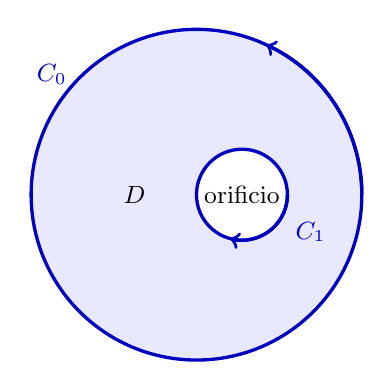
\begin{tikzpicture}[scale=1.05,every node/.style={font=\small}]
    \fill[blue!9,even odd rule] (0,0) circle (2) (.55,0) circle (.55);
    \draw[blue!75!black,very thick] (0,0) circle (2);
    \draw[blue!75!black,very thick] (.55,0) circle (.55);
    \draw[->,blue!75!black,very thick] (2,0) arc (0:65:2);
    \draw[->,blue!75!black,very thick] (1.1,0) arc (0:-105:.55);
    \node at (-.75,0) {$D$};
    \node[blue!75!black] at (-1.75,1.45) {$C_0$};
    \node[blue!75!black,right] at (1.08,-.45) {$C_1$};
    \node at (.55,0) {orificio};
\end{tikzpicture}
\end{center}
\endgroup

En la figura, $\partial D=C_0\cup C_1$. Las orientaciones opuestas hacen que $D$ quede a la izquierda tanto en la circunferencia exterior como en la interior.

\begin{mytheorem}{Teorema de Green}
Sea $D\subseteq\mathbb R^2$ una región acotada que puede descomponerse en un número finito de regiones que son simultáneamente de tipo I y de tipo II. Sea $C=\partial D$ su frontera orientada positivamente, cuyas componentes son simples y suaves por partes. Si $P$ y $Q$ tienen derivadas parciales continuas en un conjunto abierto que contiene a $D$, entonces
\[
\oint_C P\,dx+Q\,dy
=\iint_D\left(\frac{\partial Q}{\partial x}-
\frac{\partial P}{\partial y}\right)dA.
\]
Si $D$ tiene orificios, $C$ representa la unión de todas las componentes de la frontera con la orientación positiva correspondiente.
\end{mytheorem}

\begin{proof}
Primero se demuestra por separado la contribución de cada componente de la forma diferencial. Supóngase que $D$ es una región de tipo I,
\[
D=\{(x,y):a\leq x\leq b,\ g_1(x)\leq y\leq g_2(x)\}.
\]
Al recorrer la frontera positivamente, la curva inferior va de izquierda a derecha y la superior de derecha a izquierda. Los segmentos verticales, cuando aparecen, no contribuyen a $\int_C P\,dx$ porque en ellos $dx=0$. Por tanto,
\begin{align*}
\oint_C P\,dx
&=\int_a^b P(x,g_1(x))\,dx
  +\int_b^a P(x,g_2(x))\,dx\\
&=-\int_a^b\bigl(P(x,g_2(x))-P(x,g_1(x))\bigr)\,dx\\
&=-\int_a^b\int_{g_1(x)}^{g_2(x)}P_y(x,y)\,dy\,dx\\
&=-\iint_D P_y\,dA.
\end{align*}

Ahora supóngase que $D$ es una región de tipo II,
\[
D=\{(x,y):c\leq y\leq d,\ h_1(y)\leq x\leq h_2(y)\}.
\]
La parte derecha de la frontera se recorre de abajo hacia arriba y la izquierda de arriba hacia abajo. Las partes horizontales no contribuyen a $\int_C Q\,dy$. En consecuencia,
\begin{align*}
\oint_C Q\,dy
&=\int_c^d Q(h_2(y),y)\,dy
  +\int_d^c Q(h_1(y),y)\,dy\\
&=\int_c^d\bigl(Q(h_2(y),y)-Q(h_1(y),y)\bigr)\,dy\\
&=\int_c^d\int_{h_1(y)}^{h_2(y)}Q_x(x,y)\,dx\,dy\\
&=\iint_D Q_x\,dA.
\end{align*}

Si $D$ es simultáneamente de tipo I y II, al sumar ambas identidades se obtiene
\[
\oint_C P\,dx+Q\,dy
=\iint_D(Q_x-P_y)\,dA.
\]
Para una región que requiere varios subdominios, se aplica la identidad a cada uno y se suman los resultados. Cada arco interior compartido aparece dos veces con orientaciones opuestas, por lo que sus integrales se cancelan. Solo permanece la frontera de $D$. El mismo argumento trata los orificios: sus componentes permanecen como parte de la frontera y se recorren en sentido horario. Esto demuestra la fórmula en las regiones descritas por las hipótesis.
\end{proof}

\subsection{Interpretación y aplicaciones}

El integrando $Q_x-P_y$ es la componente vertical del rotacional del campo tridimensional $\langle P,Q,0\rangle$:
\[
\nabla\times\langle P,Q,0\rangle
=\left\langle0,0,Q_x-P_y\right\rangle.
\]
Green afirma que la circulación total sobre la frontera es la suma de esa rotación local sobre la región. Antes de aplicarlo deben comprobarse la orientación, el cierre de la curva y la regularidad del campo en toda la región, incluidos sus puntos interiores.

\paragraph{Ejemplo 1. Cálculo sencillo sobre una circunferencia}
Sea $C$ la circunferencia unitaria orientada en sentido antihorario. Se desea calcular
\[
\oint_C (x^2-y)\,dx+(x+y^2)\,dy.
\]
Aquí $P=x^2-y$ y $Q=x+y^2$, de modo que
\[
Q_x-P_y=1-(-1)=2.
\]
Si $D$ es el disco unitario, Green da
\[
\oint_C (x^2-y)\,dx+(x+y^2)\,dy
=\iint_D2\,dA=2\operatorname{area}(D)=2\pi.
\]

\begingroup
\shorthandoff{>}
\begin{center}
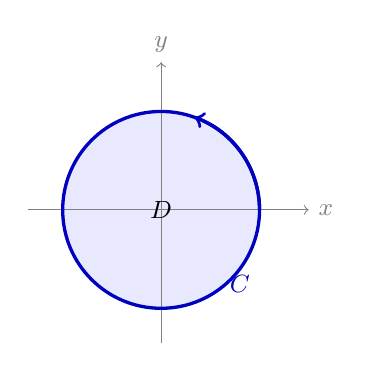
\begin{tikzpicture}[scale=1.25,every node/.style={font=\small}]
    \fill[blue!9] (0,0) circle (1);
    \draw[->,gray] (-1.35,0)--(1.5,0) node[right] {$x$};
    \draw[->,gray] (0,-1.35)--(0,1.5) node[above] {$y$};
    \draw[blue!75!black,very thick] (0,0) circle (1);
    \draw[->,blue!75!black,very thick] (1,0) arc (0:70:1);
    \node at (0,0) {$D$};
    \node[blue!75!black] at (.8,-.75) {$C$};
\end{tikzpicture}
\end{center}
\endgroup

\paragraph{Ejemplo 2. Trabajo alrededor de un rectángulo}
Sea $\mathbf{F}(x,y)=\langle x-y,x+y\rangle$ y sea $C$ la frontera positiva del rectángulo $D=[0,2]\times[0,1]$. El trabajo realizado en una vuelta completa es
\[
W=\oint_C\mathbf{F}\cdot d\vec r
=\oint_C(x-y)\,dx+(x+y)\,dy.
\]
Como $Q_x=1$ y $P_y=-1$,
\[
W=\iint_D2\,dA=2(2)(1)=4.
\]

\begingroup
\shorthandoff{>}
\begin{center}
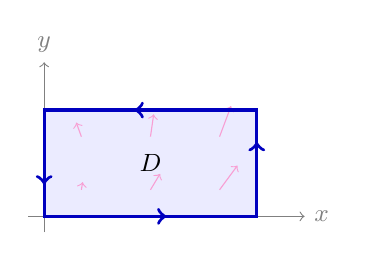
\begin{tikzpicture}[x=1.35cm,y=1.35cm,every node/.style={font=\small}]
    \fill[blue!8] (0,0) rectangle (2,1);
    \draw[->,gray] (-.15,0)--(2.45,0) node[right] {$x$};
    \draw[->,gray] (0,-.15)--(0,1.45) node[above] {$y$};
    \foreach \xx in {.35,1,1.65} {
        \foreach \yy in {.25,.75} {
            \draw[->,magenta!38!white,thin] (\xx,\yy)
                -- ++({.12*(\xx-\yy)},{.12*(\xx+\yy)});
        }
    }
    \draw[blue!75!black,very thick] (0,0)--(2,0)--(2,1)--(0,1)--cycle;
    \draw[->,blue!75!black,very thick] (.65,0)--(1.15,0);
    \draw[->,blue!75!black,very thick] (2,.25)--(2,.7);
    \draw[->,blue!75!black,very thick] (1.35,1)--(.85,1);
    \draw[->,blue!75!black,very thick] (0,.75)--(0,.3);
    \node at (1,.5) {$D$};
\end{tikzpicture}
\end{center}
\endgroup

Evaluar directamente exigiría cuatro parametrizaciones. Green reúne los cuatro tramos en una sola integral doble.

\paragraph{Ejemplo 3. Green y los campos conservativos}
Considérese
\[
\mathbf{F}(x,y)=\langle2xy+\cos x,x^2+2y\rangle.
\]
Para cualquier curva simple, cerrada y suave por partes $C$ en $\mathbb R^2$, orientada positivamente, se tiene
\[
Q_x-P_y=2x-2x=0.
\]
Por el teorema de Green,
\[
\oint_C\mathbf{F}\cdot d\vec r=\iint_D0\,dA=0.
\]
Como el campo está definido en la región simplemente conexa $\mathbb R^2$, la integral nula sobre toda curva cerrada implica independencia de la trayectoria. En efecto,
\[
\varphi(x,y)=x^2y+\sin x+y^2
\]
satisface $\nabla\varphi=\mathbf{F}$. Green proporciona así un criterio para reconocer campos conservativos en regiones sin orificios: si $P_y=Q_x$ y las derivadas son continuas, las integrales sobre curvas cerradas se anulan.

\paragraph{Ejemplo 4. Una frontera suave por partes}
Sea $C$ el triángulo orientado positivamente con vértices $(0,0)$, $(2,0)$ y $(0,1)$, y calcúlese
\[
\oint_C y^2\,dx+x^2\,dy.
\]
La frontera tiene tres segmentos suaves y tres esquinas, por lo que es suave por partes. Para $P=y^2$ y $Q=x^2$ se tiene $Q_x-P_y=2x-2y$. La región triangular puede escribirse como
\[
D=\{(x,y):0\leq x\leq2,\ 0\leq y\leq1-x/2\}.
\]
Por tanto,
\begin{align*}
\oint_C y^2\,dx+x^2\,dy
&=\int_0^2\int_0^{1-x/2}(2x-2y)\,dy\,dx\\
&=\int_0^2\left(3x-1-\frac54x^2\right)dx
=\frac23.
\end{align*}

\begingroup
\shorthandoff{>}
\begin{center}
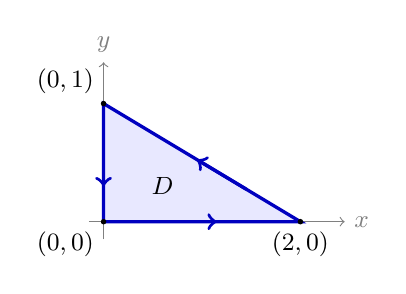
\begin{tikzpicture}[x=1.25cm,y=1.5cm,every node/.style={font=\small}]
    \fill[blue!9] (0,0)--(2,0)--(0,1)--cycle;
    \draw[->,gray] (-.15,0)--(2.45,0) node[right] {$x$};
    \draw[->,gray] (0,-.15)--(0,1.35) node[above] {$y$};
    \draw[blue!75!black,very thick] (0,0)--(2,0)--(0,1)--cycle;
    \draw[->,blue!75!black,very thick] (.6,0)--(1.15,0);
    \draw[->,blue!75!black,very thick] (1.45,.275)--(.95,.525);
    \draw[->,blue!75!black,very thick] (0,.72)--(0,.3);
    \fill (0,0) circle (1pt) node[below left] {$(0,0)$};
    \fill (2,0) circle (1pt) node[below] {$(2,0)$};
    \fill (0,1) circle (1pt) node[above left] {$(0,1)$};
    \node at (.6,.3) {$D$};
\end{tikzpicture}
\end{center}
\endgroup

La orientación de los tres segmentos es necesaria: invertir toda la trayectoria cambiaría el resultado a $-2/3$.

\subsection{Área mediante una integral de línea}

Sea $C=\partial D$ una curva simple, cerrada, suave por partes y orientada positivamente. Para calcular el área se busca que el integrando doble de Green sea igual a $1$. Tres elecciones útiles son
\[
(P,Q)=(0,x),\qquad(P,Q)=(-y,0),\qquad
(P,Q)=\left(-\frac y2,\frac x2\right).
\]
De ellas se obtienen las fórmulas
\begin{mytheorem}{Fórmulas de área con integrales de línea}
\[
\operatorname{area}(D)
=\oint_C x\,dy
=-\oint_C y\,dx
=\frac12\oint_C(x\,dy-y\,dx).
\]
Si $\vec r(t)=(x(t),y(t))$, $a\leq t\leq b$, recorre $C$ una vez en sentido positivo, entonces
\[
\operatorname{area}(D)
=\frac12\int_a^b\bigl(x(t)y'(t)-y(t)x'(t)\bigr)\,dt.
\]
\end{mytheorem}

Estas fórmulas producen área con signo: una orientación negativa cambia el signo de la integral. En una región con orificios deben incluirse todas las componentes de la frontera con su orientación positiva.

\paragraph{Ejemplo 5. Área de una elipse}
La elipse
\[
\frac{x^2}{a^2}+\frac{y^2}{b^2}=1,
\qquad a,b>0,
\]
se parametriza en sentido antihorario mediante $x(t)=a\cos t$, $y(t)=b\sin t$, $0\leq t\leq2\pi$. Por la fórmula simétrica,
\begin{align*}
\operatorname{area}(D)
&=\frac12\int_0^{2\pi}
\left(a\cos t\,b\cos t-b\sin t(-a\sin t)\right)dt\\
&=\frac{ab}{2}\int_0^{2\pi}1\,dt
=\pi ab.
\end{align*}

\begingroup
\shorthandoff{>}
\begin{center}
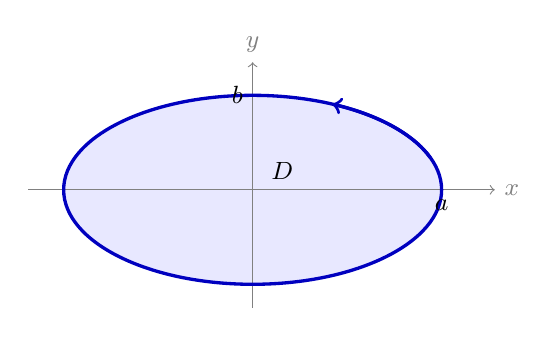
\begin{tikzpicture}[x=1.5cm,y=1.2cm,every node/.style={font=\small}]
    \fill[blue!9] (0,0) ellipse (1.6 and 1);
    \draw[->,gray] (-1.9,0)--(2.05,0) node[right] {$x$};
    \draw[->,gray] (0,-1.25)--(0,1.35) node[above] {$y$};
    \draw[blue!75!black,very thick] (0,0) ellipse (1.6 and 1);
    \draw[->,blue!75!black,very thick]
        ({1.6*cos(20)},{sin(20)}) arc[start angle=20,end angle=65,x radius=1.6,y radius=1];
    \node[below] at (1.6,0) {$a$};
    \node[left] at (0,1) {$b$};
    \node at (.25,.2) {$D$};
\end{tikzpicture}
\end{center}
\endgroup

\paragraph{Ejemplo 6. Área de una región con un orificio}
Sea $D$ la región comprendida entre las circunferencias concéntricas de radios $R$ y $r$, con $0<r<R$. La frontera exterior $C_R$ se recorre en sentido antihorario y la interior $C_r$ en sentido horario. Para $C_R$ se usa
\[
(x,y)=(R\cos t,R\sin t),\qquad0\leq t\leq2\pi,
\]
mientras que una parametrización positiva de $C_r$ es
\[
(x,y)=(r\cos t,-r\sin t),\qquad0\leq t\leq2\pi.
\]
La fórmula simétrica produce
\begin{align*}
\operatorname{area}(D)
&=\frac12\int_{C_R}(x\,dy-y\,dx)
 +\frac12\int_{C_r}(x\,dy-y\,dx)\\
&=\frac12\int_0^{2\pi}R^2\,dt
  +\frac12 + \int_0^{2\pi}(-r^2)\,dt\\
&=\pi(R^2-r^2).
\end{align*}

\begingroup
\shorthandoff{>}
\begin{center}
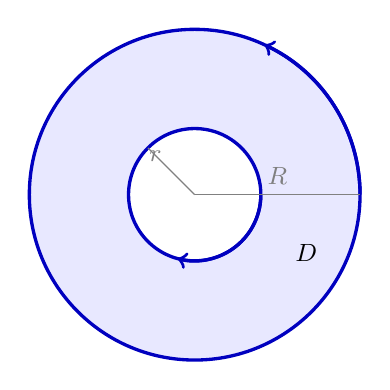
\begin{tikzpicture}[scale=1.05,every node/.style={font=\small}]
    \fill[blue!9,even odd rule] (0,0) circle (2) (0,0) circle (.8);
    \draw[blue!75!black,very thick] (0,0) circle (2);
    \draw[blue!75!black,very thick] (0,0) circle (.8);
    \draw[->,blue!75!black,very thick] (2,0) arc (0:65:2);
    \draw[->,blue!75!black,very thick] (.8,0) arc (0:-105:.8);
    \draw[gray] (0,0)--(2,0) node[midway,above] {$R$};
    \draw[gray] (0,0)--({.8*cos(135)},{.8*sin(135)})
        node[midway,above left] {$r$};
    \node at (1.35,-.7) {$D$};
\end{tikzpicture}
\end{center}
\endgroup

La contribución negativa de la frontera interior resta automáticamente el área del orificio.

\subsection{Formas alternativas del teorema de Green}

\paragraph{Forma de circulación}
Si $\mathbf{F}=\langle P,Q\rangle$ y $\mathbf{T}$ es la tangente unitaria orientada positivamente, entonces $d\vec r=\mathbf{T}\,ds$ y
\[
\oint_C\mathbf{F}\cdot\mathbf{T}\,ds
=\oint_C\mathbf{F}\cdot d\vec r
=\iint_D(Q_x-P_y)\,dA.
\]
Al identificar $\mathbf{F}$ con $\langle P,Q,0\rangle$ y usar $\mathbf{k}=\langle0,0,1\rangle$, también se escribe
\[
\oint_C\mathbf{F}\cdot d\vec r
=\iint_D(\nabla\times\mathbf{F})\cdot\mathbf{k}\,dA.
\]

\paragraph{Forma de flujo}
Sea $\vec r(s)=\langle x(s),y(s)\rangle$ una parametrización por longitud de arco de una componente de $C$, recorrida con orientación positiva. Como $s$ mide longitud, el vector
\[
\mathbf{T}(s)=\vec r\,'(s)
=\left\langle\frac{dx}{ds},\frac{dy}{ds}\right\rangle
\]
es tangente a la curva y tiene norma $1$. Al avanzar sobre $C$, la región $D$ permanece a la izquierda de $\mathbf{T}$. En consecuencia, el exterior queda a su derecha. La normal unitaria exterior se obtiene al girar $\mathbf{T}$ un ángulo de $90^\circ$ en sentido horario:
\[
\mathbf{n}=\left\langle\frac{dy}{ds},-\frac{dx}{ds}\right\rangle.
\]
Este vector también tiene norma $1$, pues
\[
\lVert\mathbf{n}\rVert^2
=\left(\frac{dy}{ds}\right)^2+
  \left(\frac{dx}{ds}\right)^2
=\lVert\mathbf{T}\rVert^2=1.
\]

\begingroup
\shorthandoff{>}
\begin{center}
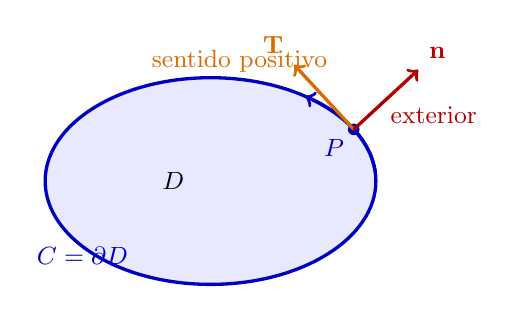
\begin{tikzpicture}[scale=1.05,every node/.style={font=\small}]
    \fill[blue!9] (0,0) ellipse (2 and 1.25);
    \draw[blue!75!black,very thick] (0,0) ellipse (2 and 1.25);
    \draw[->,blue!75!black,very thick]
        ({2*cos(5)},{1.25*sin(5)})
        arc[start angle=5,end angle=55,x radius=2,y radius=1.25];
    \coordinate (P) at ({2*cos(30)},{1.25*sin(30)});
    \fill[blue!75!black] (P) circle (2pt) node[below left] {$P$};
    \draw[->,orange!85!black,very thick] (P) -- ++(-.72,.78)
        node[above left] {$\mathbf{T}$};
    \draw[->,red!70!black,very thick] (P) -- ++(.78,.72)
        node[above right] {$\mathbf{n}$};
    \draw[red!55!black,dashed] (P) -- ++(.38,.35);
    \node at (-.45,0) {$D$};
    \node[blue!75!black] at (-1.55,-.9) {$C=\partial D$};
    \node[orange!85!black] at (.35,1.45) {sentido positivo};
    \node[red!70!black] at (2.7,.8) {exterior};
\end{tikzpicture}
\end{center}
\endgroup

La figura muestra que $\mathbf{T}$ sigue el sentido positivo de la frontera, mientras que $\mathbf{n}$ apunta hacia afuera de $D$. El producto punto $\mathbf{F}\cdot\mathbf{n}$ mide la componente normal del campo: es positivo donde el campo sale de la región, negativo donde entra y cero donde es tangente a la frontera. Al multiplicarlo por el elemento de longitud $ds$ se obtiene el flujo a través de un arco infinitesimal.

El elemento normal dirigido satisface
\[
\mathbf{n}\,ds
=\left\langle dy,-dx\right\rangle.
\]
Por tanto, si $\mathbf{F}=\langle P,Q\rangle$,
\[
\mathbf{F}\cdot\mathbf{n}\,ds=P\,dy-Q\,dx.
\]
Para una parametrización cualquiera $\vec r(t)=\langle x(t),y(t)\rangle$, $a\leq t\leq b$, que recorre positivamente la frontera, la misma expresión toma la forma
\[
\mathbf{n}\,ds=\langle y'(t),-x'(t)\rangle\,dt,
\]
y, por consiguiente,
\[
\oint_C\mathbf{F}\cdot\mathbf{n}\,ds
=\int_a^b\left[P(x(t),y(t))y'(t)
-Q(x(t),y(t))x'(t)\right]dt.
\]

Al aplicar la forma de circulación al campo $\langle-Q,P\rangle$ se obtiene
\[
\oint_C\mathbf{F}\cdot\mathbf{n}\,ds
=\oint_C P\,dy-Q\,dx
=\iint_D(P_x+Q_y)\,dA
=\iint_D\nabla\cdot\mathbf{F}\,dA.
\]
Esta forma expresa que el flujo neto hacia afuera de la frontera es igual a la suma de la divergencia dentro de la región.


\subsection{Ejercicios}
\begin{enumerate}
    \item Determine si cada recorrido tiene orientación positiva o negativa respecto de la región que encierra. Indique cómo cambia el signo de una integral de línea si se invierte el sentido.
\begin{enumerate}
    \item Una circunferencia recorrida en sentido antihorario.
    \item La frontera exterior de una región recorrida en sentido horario.
    \item La frontera de un orificio recorrida en sentido horario, mientras la frontera exterior se recorre en sentido antihorario.
\end{enumerate}

    \item Use el teorema de Green para evaluar
\[
\oint_C y\,dx-x\,dy,
\]
donde $C$ es la circunferencia unitaria orientada en sentido antihorario.

    \item Sea $C$ la frontera positiva del rectángulo $0\leq x\leq2$, $0\leq y\leq3$. Evalúe
\[
\oint_C xy\,dx+(x^2+y)\,dy
\]
mediante una integral doble.

    \item Sea $C$ la frontera positiva del triángulo con vértices $(0,0)$, $(2,0)$ y $(0,2)$. Calcule
\[
\oint_C xy\,dx+x^2\,dy
\]
usando el teorema de Green.

    \item Para $\mathbf{F}(x,y)=\langle x-y,x+y\rangle$ y la circunferencia unitaria $C$ orientada en sentido antihorario, calcule $\oint_C\mathbf{F}\cdot d\vec r$ de dos maneras: mediante la parametrización $\vec r(t)=(\cos t,\sin t)$ y mediante el teorema de Green.

    \item Una partícula recorre en sentido antihorario la elipse $x^2/a^2+y^2/b^2=1$, donde $a,b>0$, bajo el campo
\[
\mathbf{F}(x,y)=\left\langle-\frac y2,\frac x2\right\rangle.
\]
Use el teorema de Green para calcular el trabajo realizado en una vuelta completa e interprete su relación con el área encerrada.

    \item La curva $C$ recorre positivamente el polígono mostrado. Use el teorema de Green para calcular
\[
\oint_C-y\,dx+x\,dy.
\]
\begingroup
\shorthandoff{>}
\begin{center}
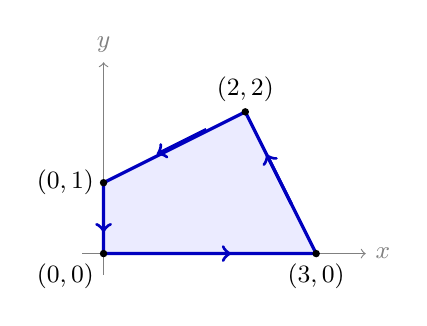
\begin{tikzpicture}[scale=.9,every node/.style={font=\small}]
    \draw[->,gray] (-.3,0)--(3.7,0) node[right] {$x$};
    \draw[->,gray] (0,-.3)--(0,2.7) node[above] {$y$};
    \fill[blue!8] (0,0)--(3,0)--(2,2)--(0,1)--cycle;
    \draw[blue!75!black,very thick] (0,0)--(3,0)--(2,2)--(0,1)--cycle;
    \draw[->,blue!75!black,very thick] (1,0)--(1.8,0);
    \draw[->,blue!75!black,very thick] (2.65,.7)--(2.3,1.4);
    \draw[->,blue!75!black,very thick] (1.45,1.75)--(.75,1.4);
    \draw[->,blue!75!black,very thick] (0,.75)--(0,.3);
    \fill (0,0) circle (1.5pt) node[below left] {$(0,0)$};
    \fill (3,0) circle (1.5pt) node[below] {$(3,0)$};
    \fill (2,2) circle (1.5pt) node[above] {$(2,2)$};
    \fill (0,1) circle (1.5pt) node[left] {$(0,1)$};
\end{tikzpicture}
\end{center}
\endgroup

    \item Sea
\[
\mathbf{F}(x,y)=\langle3x^2-2y,-2x+4y^3\rangle.
\]
Use el teorema de Green para demostrar que la integral de $\mathbf{F}$ sobre toda curva simple, cerrada y suave por partes en $\mathbb R^2$ es cero. Encuentre una función potencial y verifique el resultado con el teorema fundamental de las integrales de línea.

    \item Para $\mathbf{F}(x,y)=\langle y^2,x\rangle$, calcule con Green la circulación sobre la circunferencia unitaria orientada positivamente y decida si $\mathbf{F}$ puede ser conservativo en todo $\mathbb R^2$.

    \item La circunferencia $(x-a)^2+(y-b)^2=R^2$ se recorre en sentido antihorario. Use una fórmula de área basada en Green y la parametrización
\[
x(t)=a+R\cos t,\qquad y(t)=b+R\sin t,\qquad0\leq t\leq2\pi,
\]
para demostrar que el área encerrada no depende del centro $(a,b)$.

    \item Use una integral de línea para calcular el área encerrada por la parábola $y=x^2$ y la recta $y=2x$. Oriente positivamente la frontera y proporcione una parametrización para cada arco.

    \item La astroide se parametriza en sentido antihorario mediante
\[
x(t)=a\cos^3t,\qquad y(t)=a\sin^3t,\qquad0\leq t\leq2\pi,
\]
donde $a>0$. Use la fórmula $\frac12\oint_C(x\,dy-y\,dx)$ para determinar el área encerrada.

    \item Una región está dentro de la elipse $x^2/a^2+y^2/b^2=1$ y fuera de la circunferencia $x^2+y^2=r^2$, donde $0<r<\min\{a,b\}$. Oriente positivamente la frontera y calcule el área mediante una integral de línea.

    \item Sea $\mathbf{F}(x,y)=\langle x,y\rangle$ y sea $C$ la circunferencia unitaria. Calcule el flujo exterior
\[
\oint_C\mathbf{F}\cdot\mathbf{n}\,ds
\]
primero mediante la forma de flujo del teorema de Green y después directamente, usando que sobre $C$ se tiene $\mathbf{n}=\langle x,y\rangle$.

    \item Sea $D=\{(x,y):r^2\leq x^2+y^2\leq R^2\}$, donde $0<r<R$, y sea
\[
\mathbf{F}(x,y)=\left\langle-\frac{y}{x^2+y^2},\frac{x}{x^2+y^2}\right\rangle.
\]
Oriente positivamente $\partial D$ y calcule la circulación sobre cada componente para verificar el teorema de Green. Explique por qué no puede aplicarse al disco $x^2+y^2\leq R^2$ y por qué el campo no tiene un potencial en todo $\mathbb R^2\setminus\{(0,0)\}$, aunque su rotacional sea nulo.

\end{enumerate}
